An electron can be misidentified as a photon if the association of tracks or track seeds to the ECAL supercluster fails in the reconstruction step. 
The production of a single \PW\ boson decaying to an electron and a neutrino is a high-rate process, and it mimicks the photon plus \met\ signature if the electron is misidentified.

The rate  at which this misidentification occurs is $R_{\Pe} = (1 - \epsilon_{\Pe}^{\text{track}}) / \epsilon_{\Pe}^{\text{track}}$, where $\epsilon_{\Pe}^{\text{track}}$ is the tracking efficiency of electrons passing the photon identification criteria except for the electron veto.
After making the reasonable assumption that the kinematic and other critical properties of the electron plus \met\ events are unaffected by the electron misidentification, we model the electron misidentification background by taking the electron proxy sample and scaling it by $R_{\Pe}$.

% This partial identification is denoted as \Pe\Pgg\ ID in the following.
% The first such change is that the sample is split into \Pe\Pgg\ and \Pe\Pe\ categories depending on whether the probe passes or fails the electron veto requirement. 

We measure the factor $R_{\Pe}$ in data using the TP method described in Section~\ref{sec:idsf} with changed definitions for passing and failing probes and an adjustment to the background model.
The \Pe\Pe\ category contains passing probes with a pixel seed while the \Pe\Pgg\ category contrains failing probes without a pixel seed.
Probes in both categories must pass the remainder of the \egamma\ and \Pgg-specific IDs.
Denoting the area of the peak in each category  $N_{\Pe\Pe}$ and $N_{\Pe\Pgg}$, respectively, the ratio $N_{\Pe\Pgg} / N_{\Pe\Pe}$ is equal to $R_{\Pe}$ up to minor systematic corrections.

%%% these fils have charged PF veto included, need to swap out
\begin{figure}[htbp]
  \centering
  \resizebox{0.95\textwidth}{!}{
    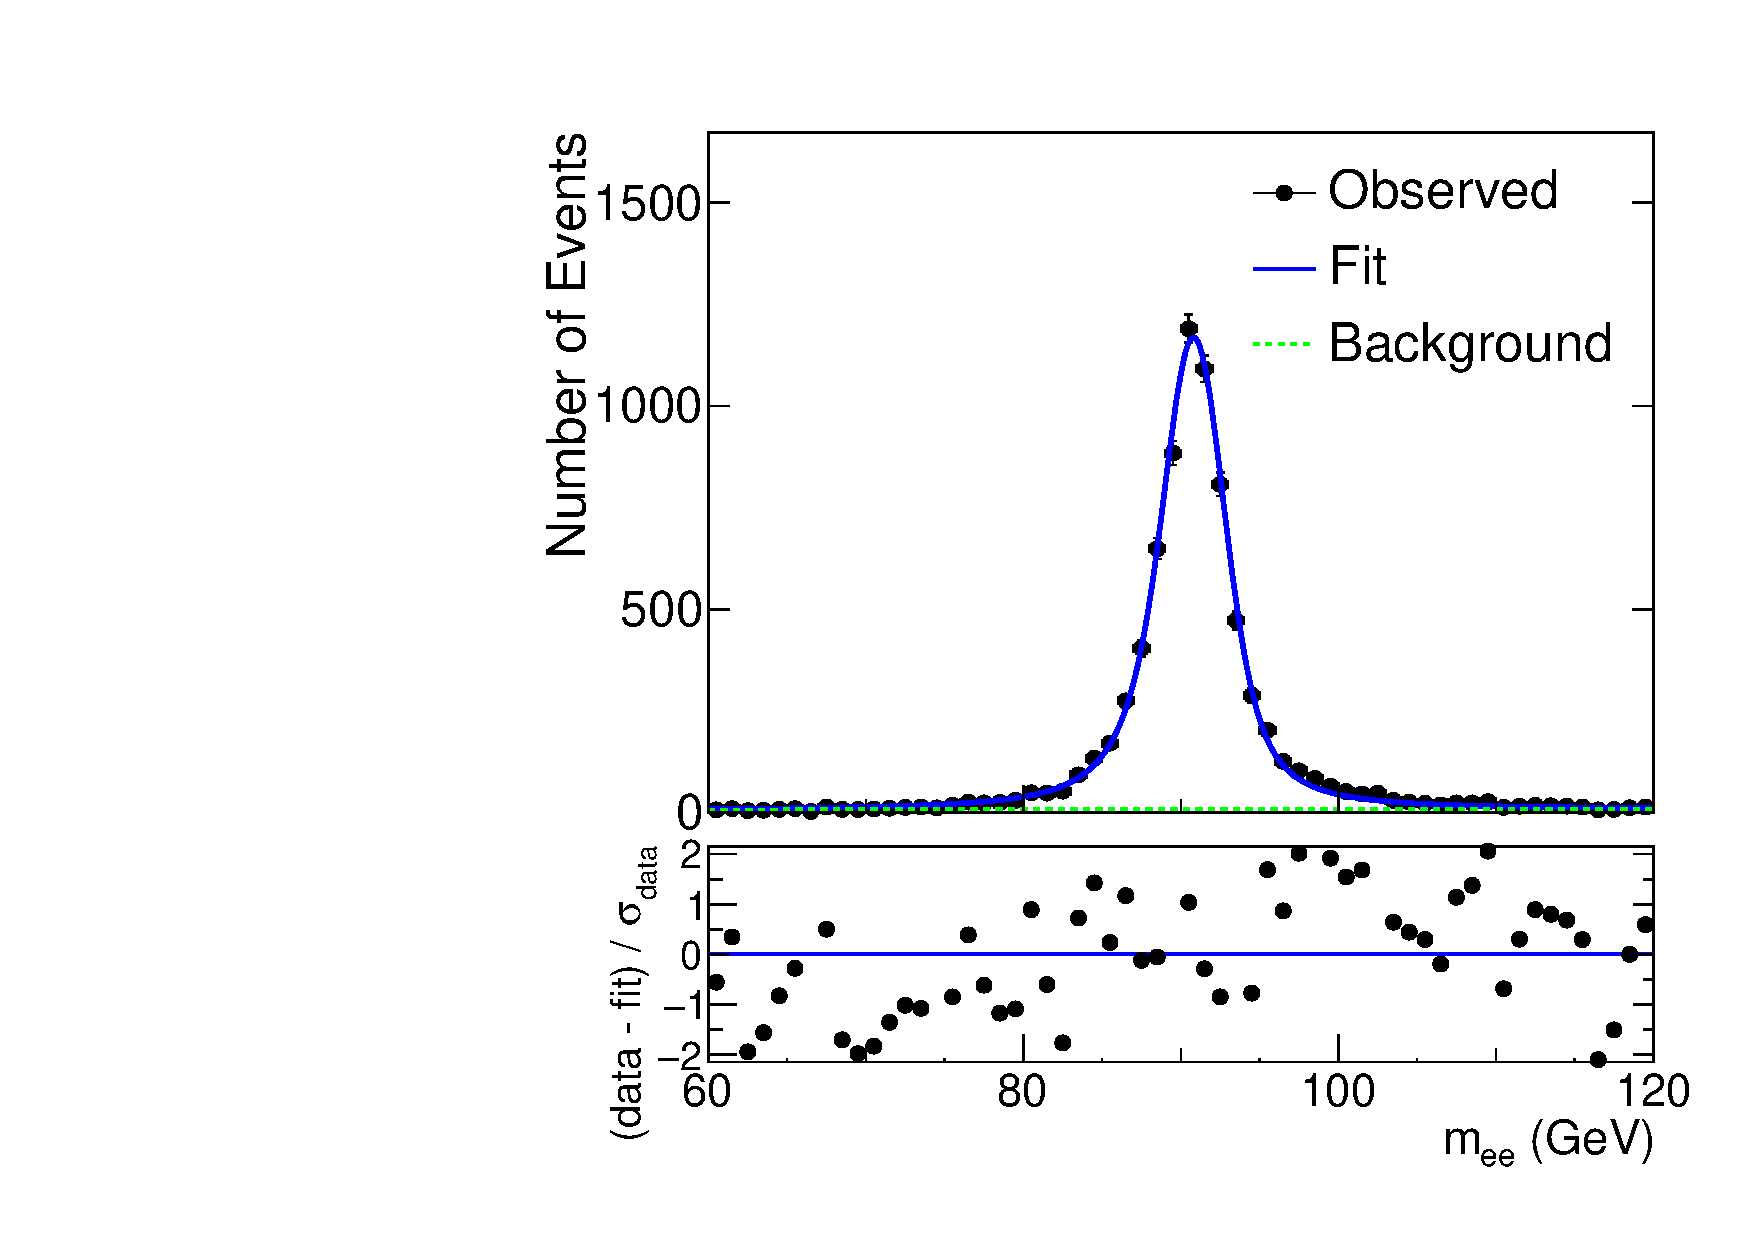
\includegraphics[]{Analysis/Figures/efake/fit_data_ee_pt_175_200.pdf}
    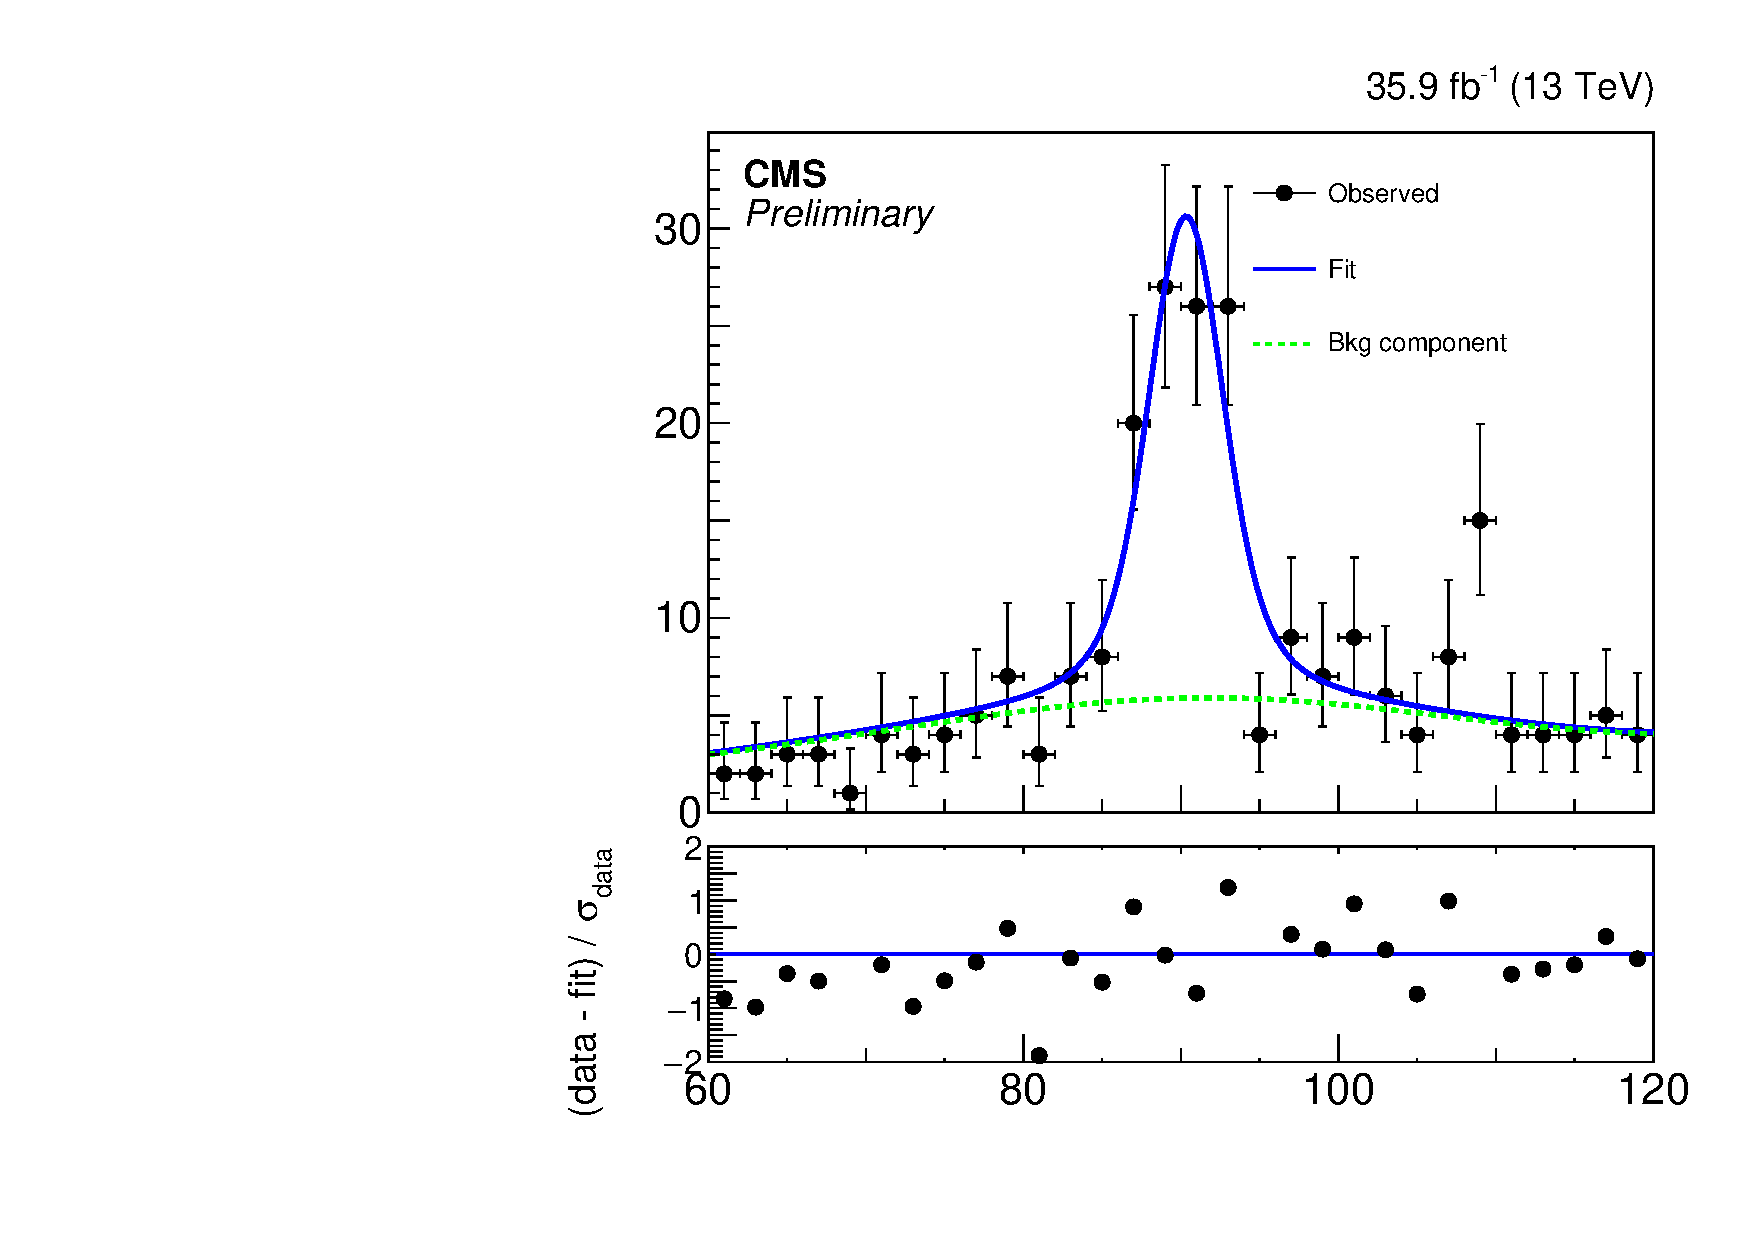
\includegraphics[]{Analysis/Figures/efake/fit_data_eg_pt_175_200.pdf}
  }
  \resizebox{0.95\textwidth}{!}{
    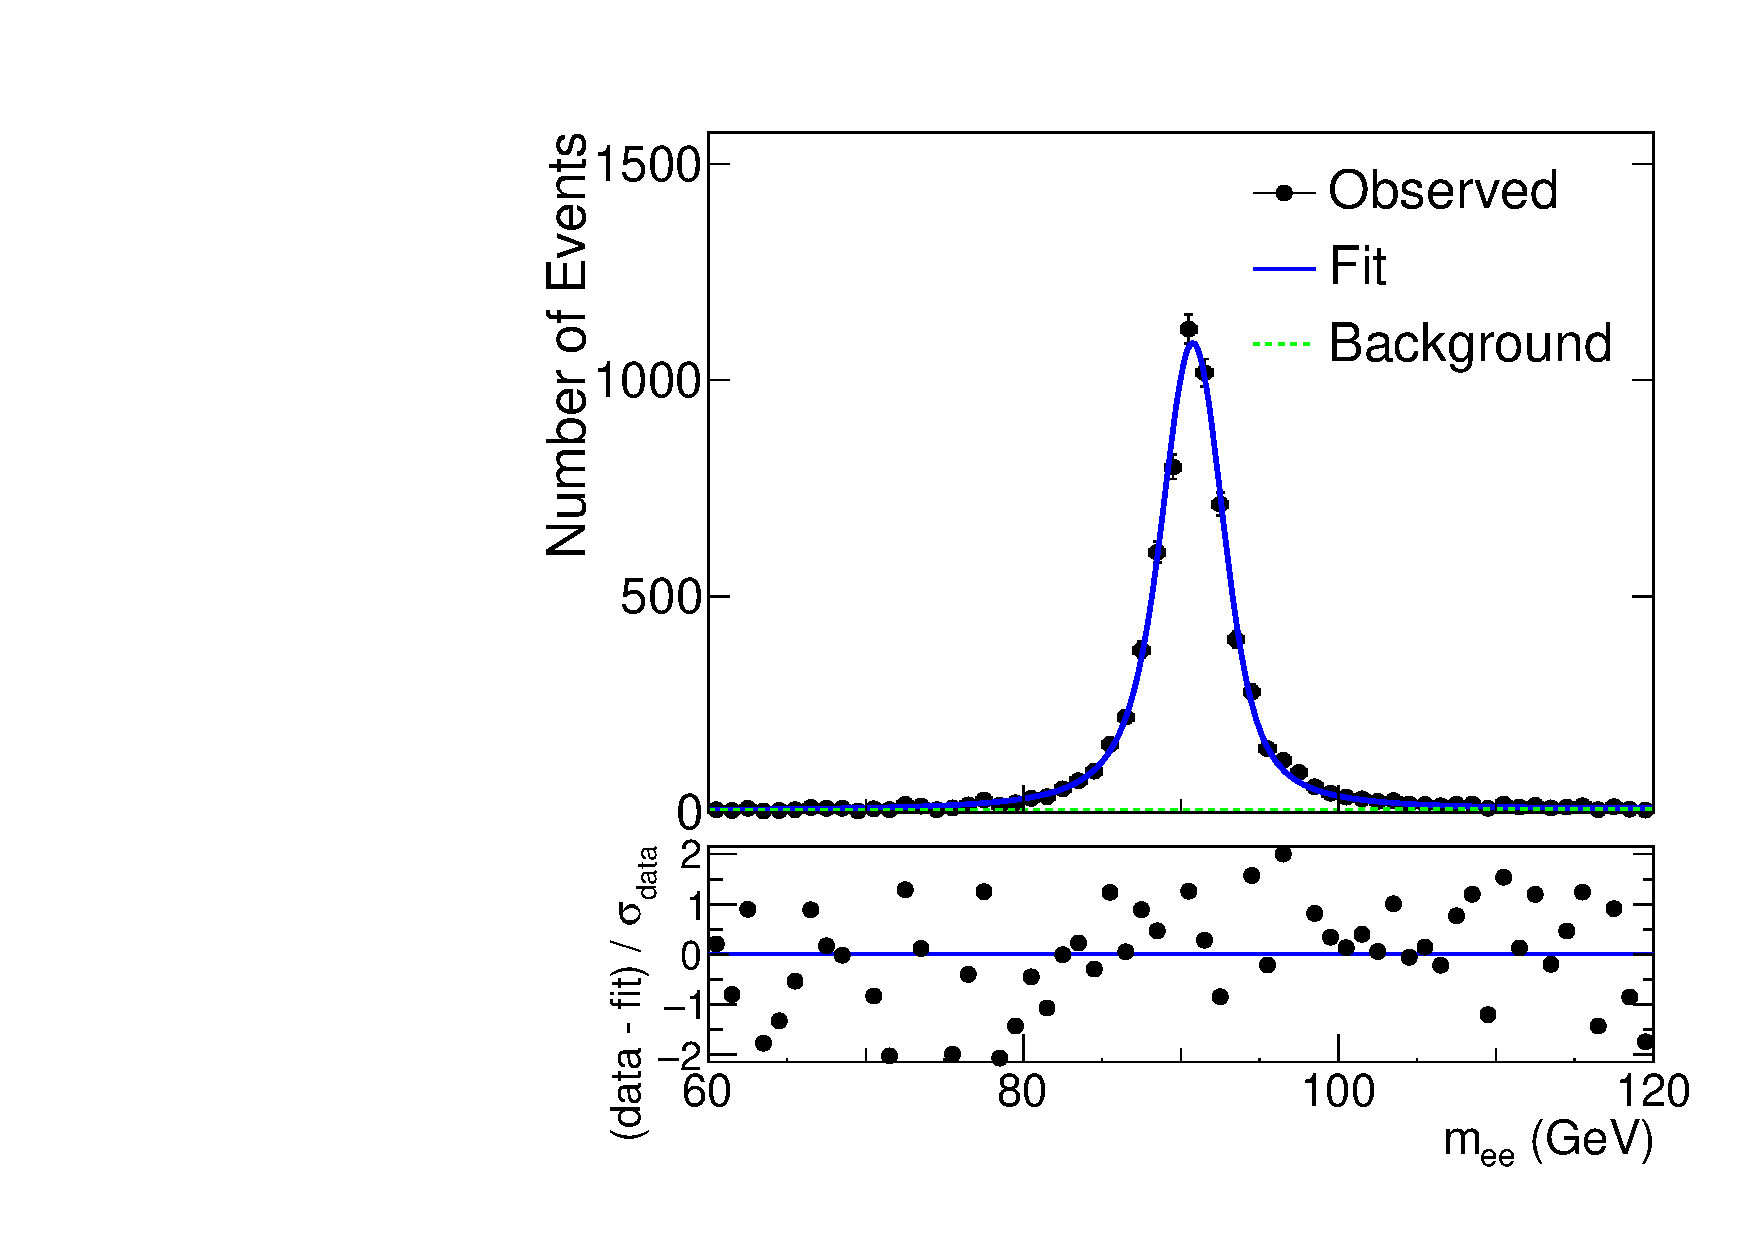
\includegraphics[]{Analysis/Figures/efake/fit_data_ee_pt_200_250.pdf}
    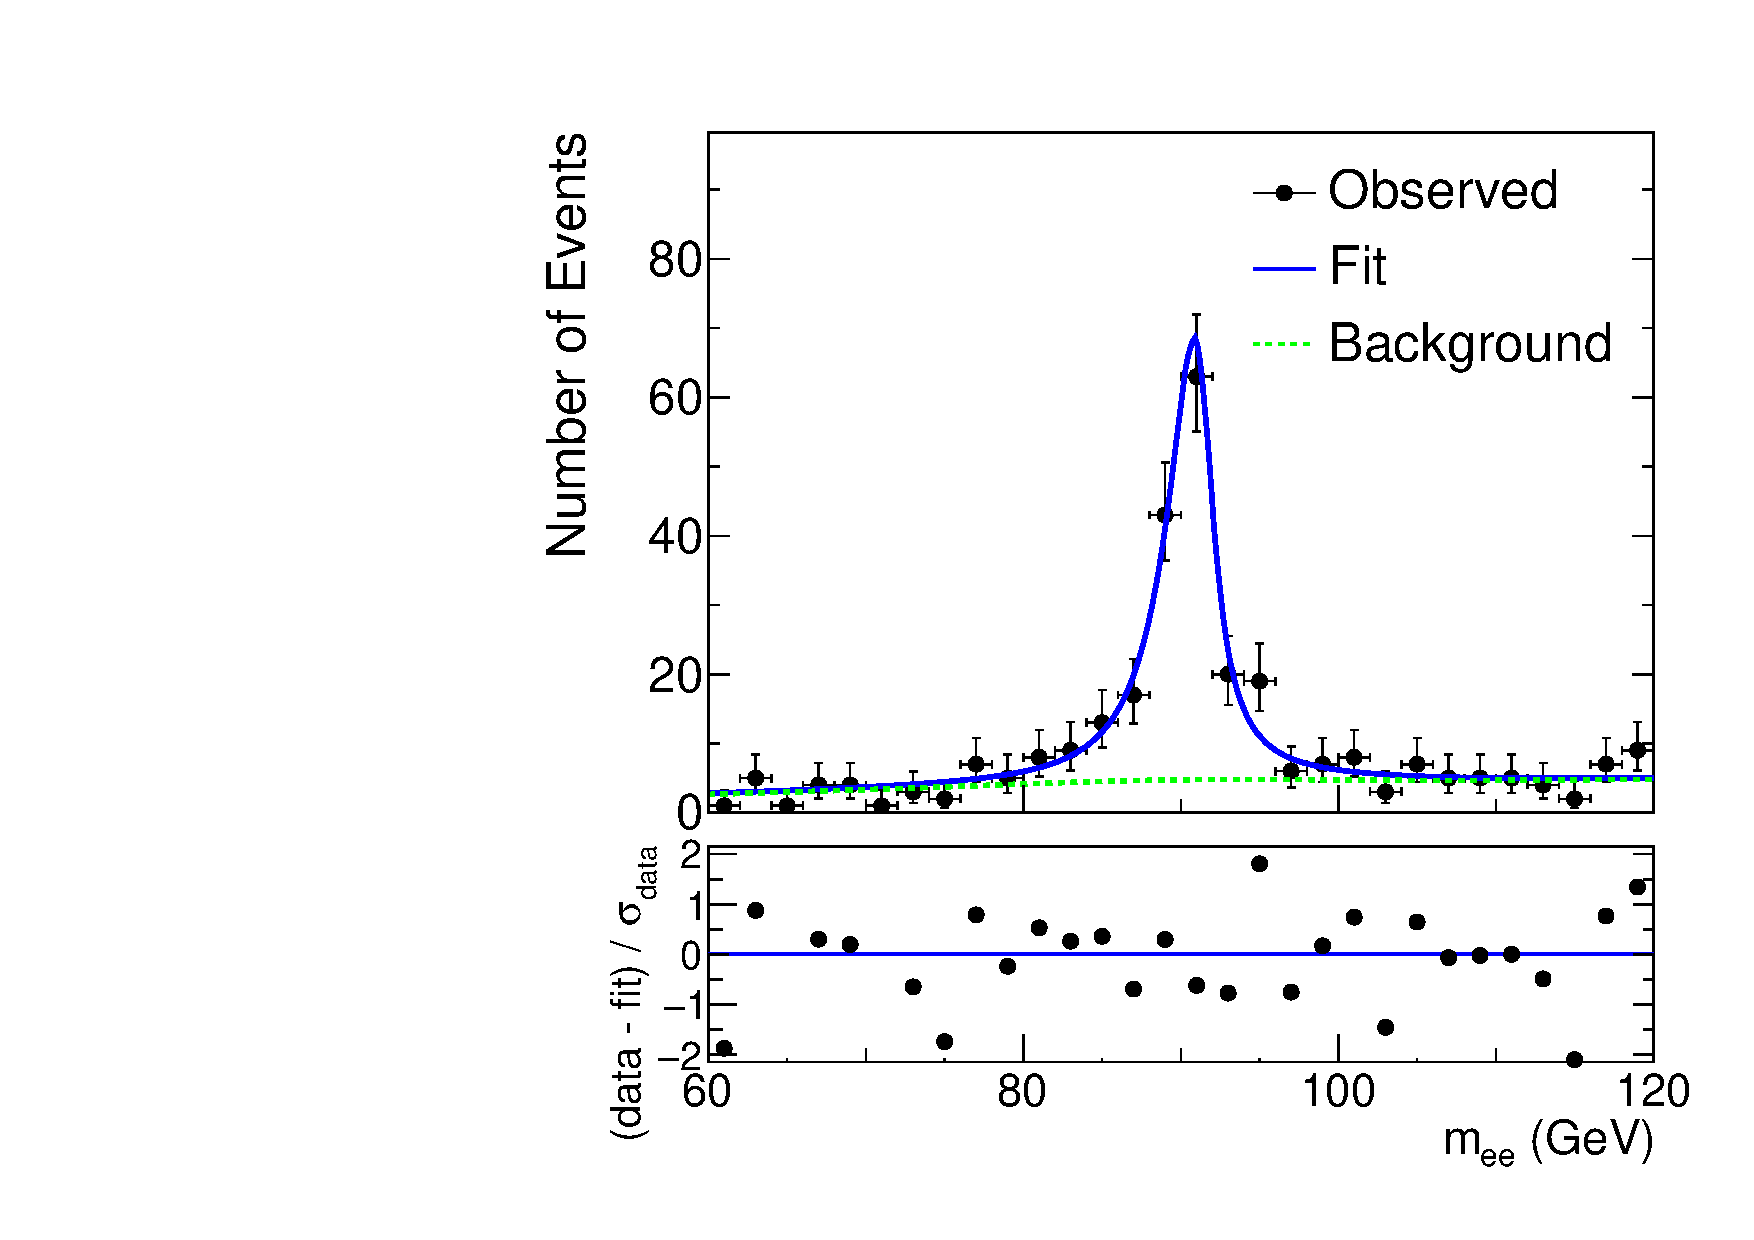
\includegraphics[]{Analysis/Figures/efake/fit_data_eg_pt_200_250.pdf}
  }
  \resizebox{0.95\textwidth}{!}{
    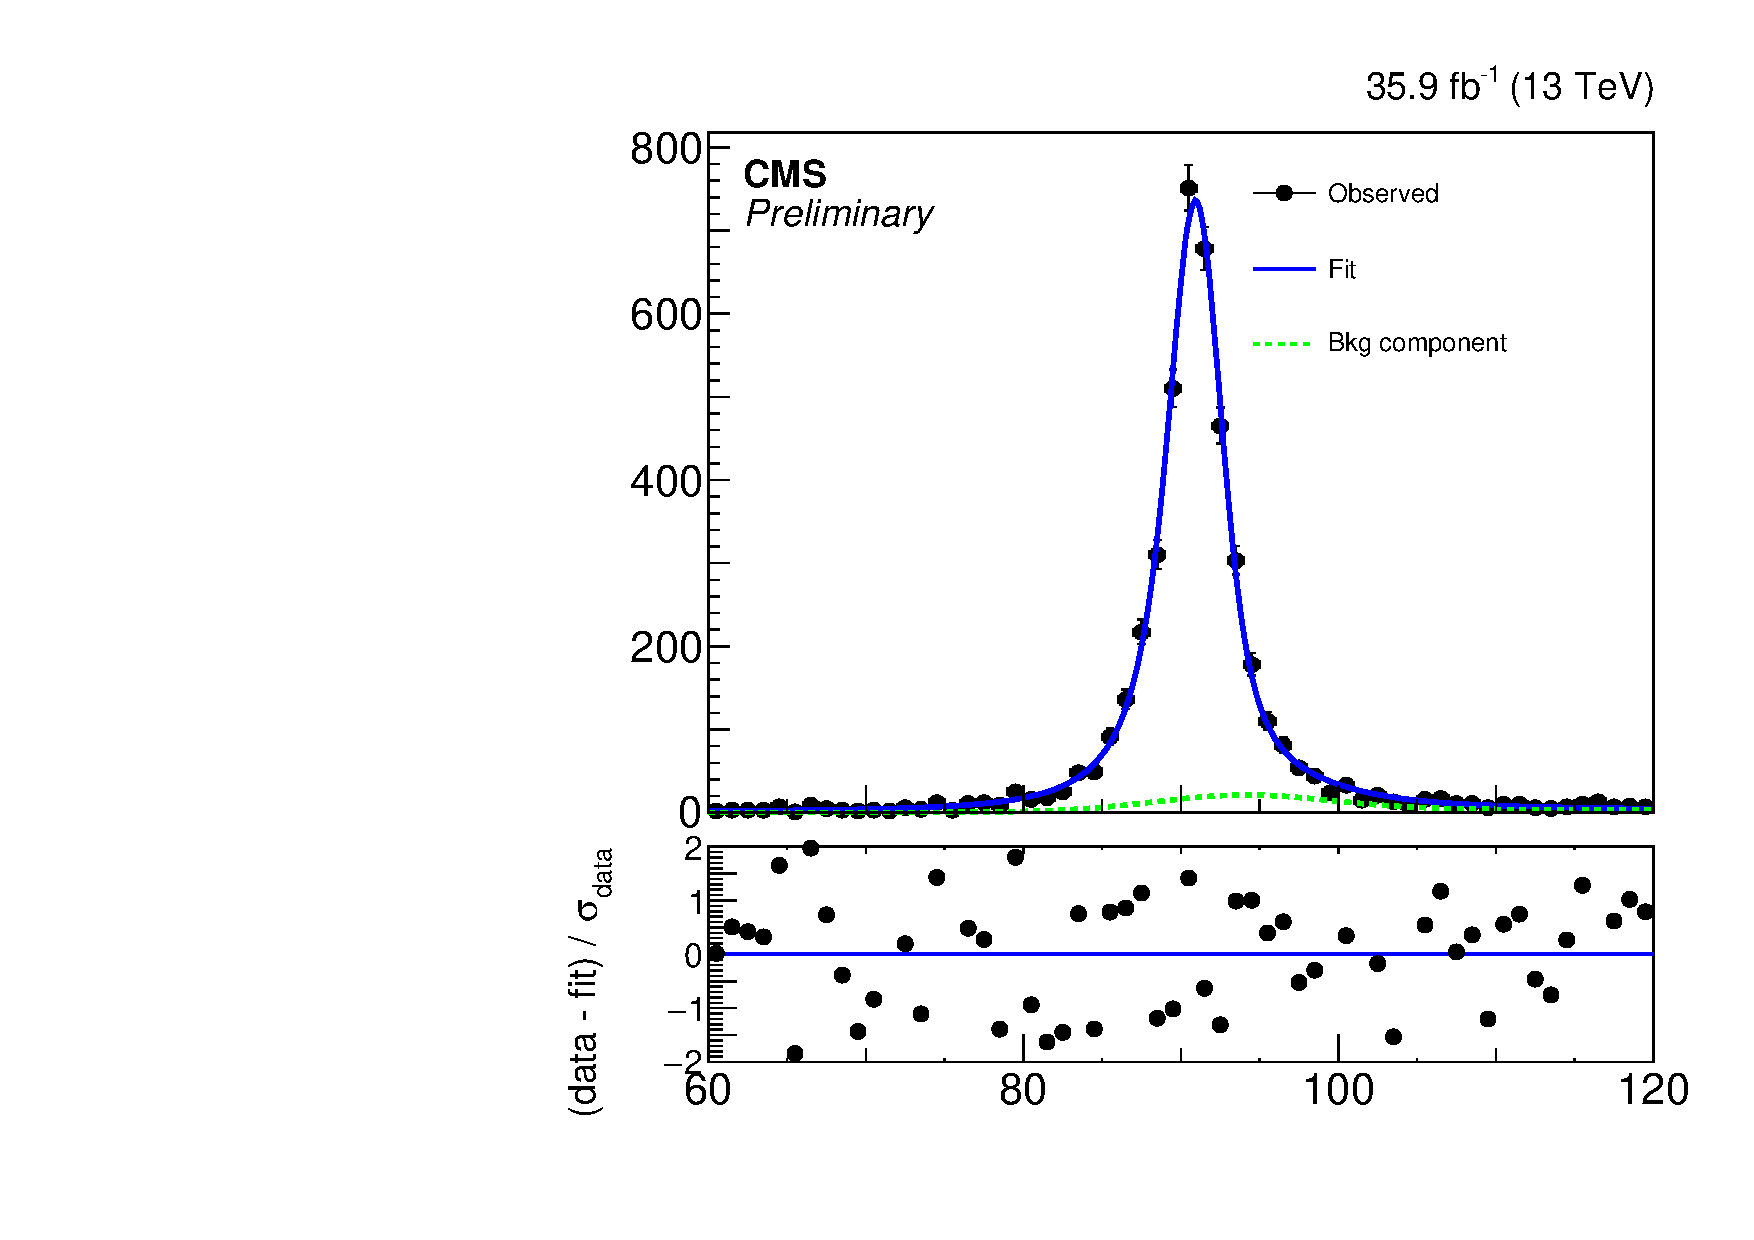
\includegraphics[]{Analysis/Figures/efake/fit_data_ee_pt_250_6500.pdf}
    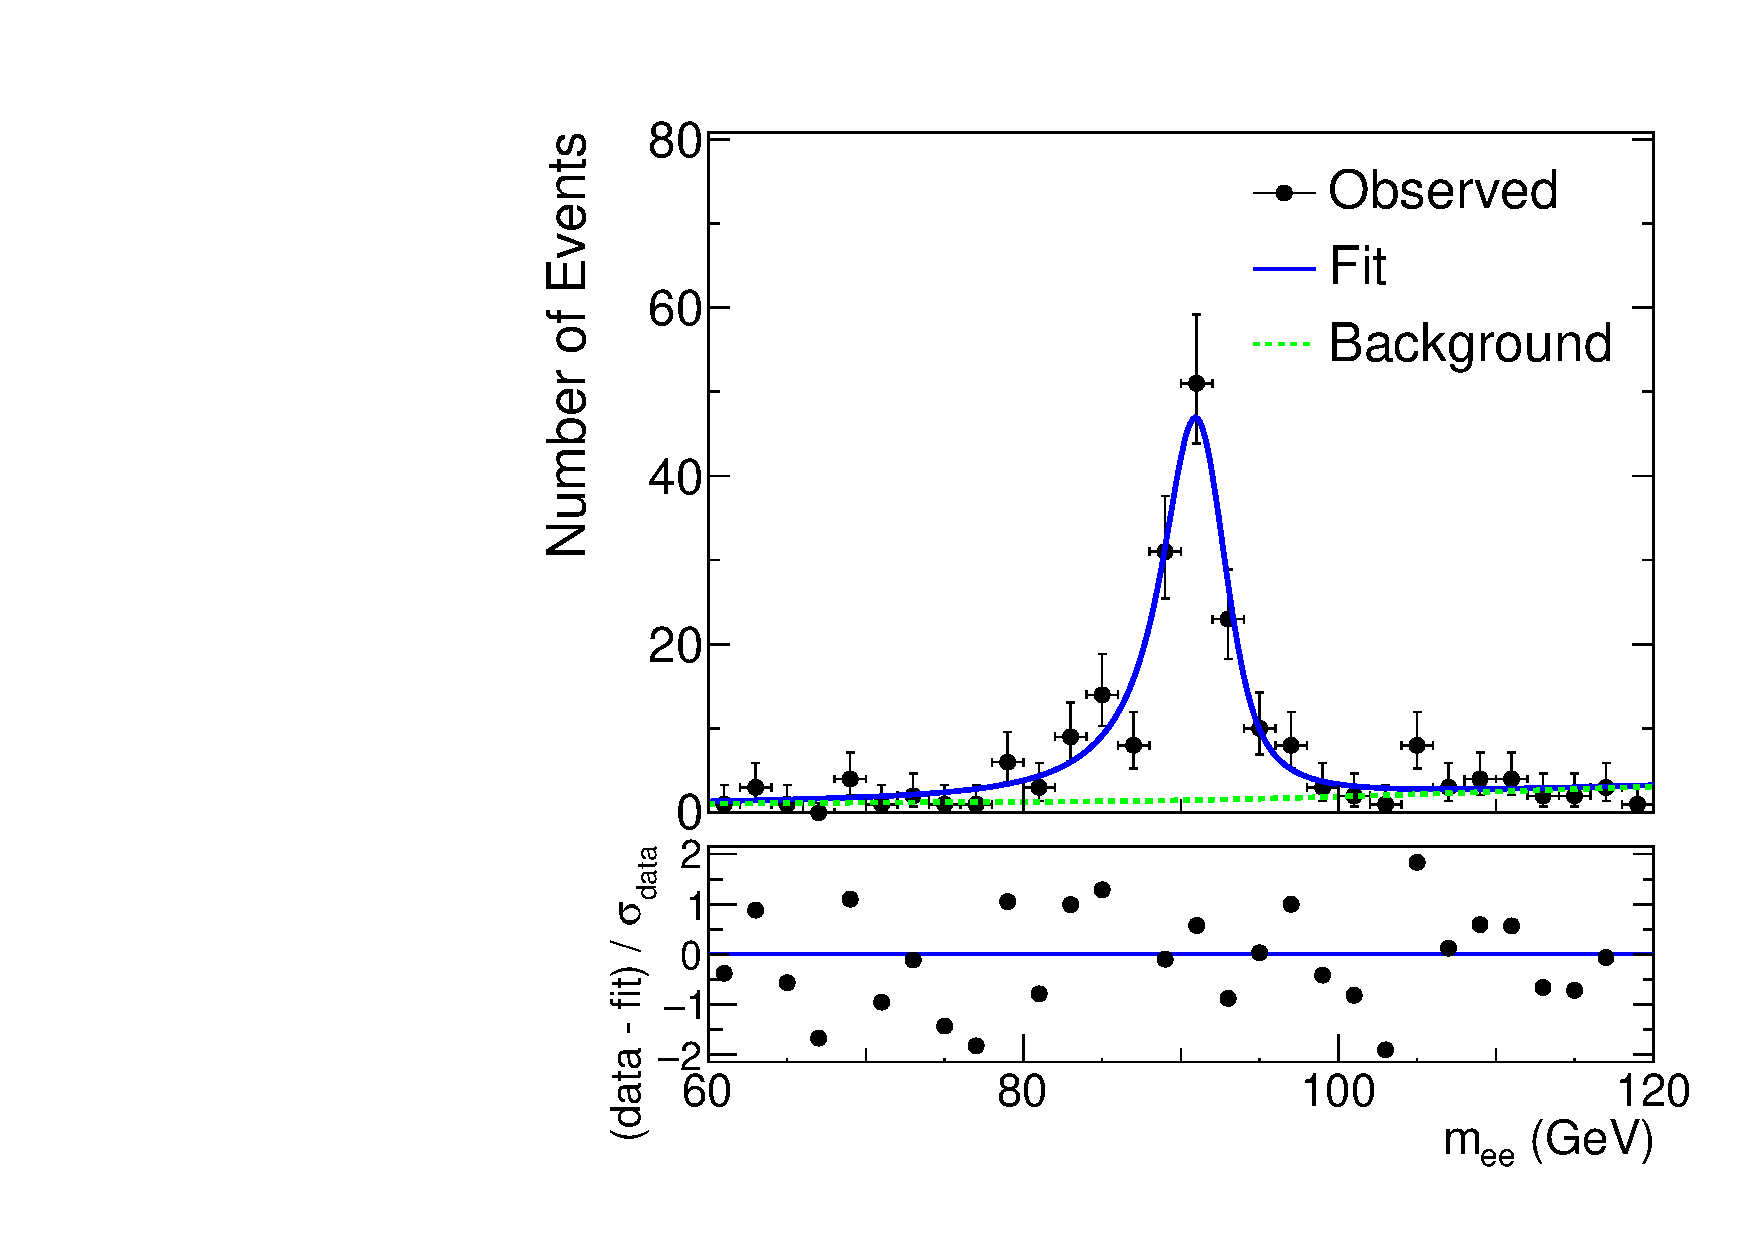
\includegraphics[]{Analysis/Figures/efake/fit_data_eg_pt_250_6500.pdf}
  }
  \caption{
      Fits to the mass distributions for \Pe\Pe\ (left) and \Pe\Pgg\ (right) selections, in bins of probe $\pt$: $175 < \pt < 200\GeV$ (top), $200 < \pt < 250\GeV$ (middle), $\pt > 250\GeV$ (bottom). 
      The blue solid line represents the full fit model, and the green dashed line its background component.
    }
    \label{fig:efake_fits}
\end{figure}

Additionally, the backgrounds to the \Pe\Pgg\ fit consist of processes with an electron and an actual photon in the final state, such as \PW\Pgg\ and \Zee\ with a hard radiation off one of the electrons.
To account for the higher rate of bremsstrahlung experienced by electrons than by muons, we scale the mass distribution of the $\Pgm+\Pgg$ sample by the ratio of electron-probe to muon-probe events taken from MC.
As an alternative template to assess the systematic effect introduced by the choice of the background template, the unscaled mass distribution is also tested.

%%% this file has charged PF veto included, need to swap out
\begin{figure}[htbp]
\centering
    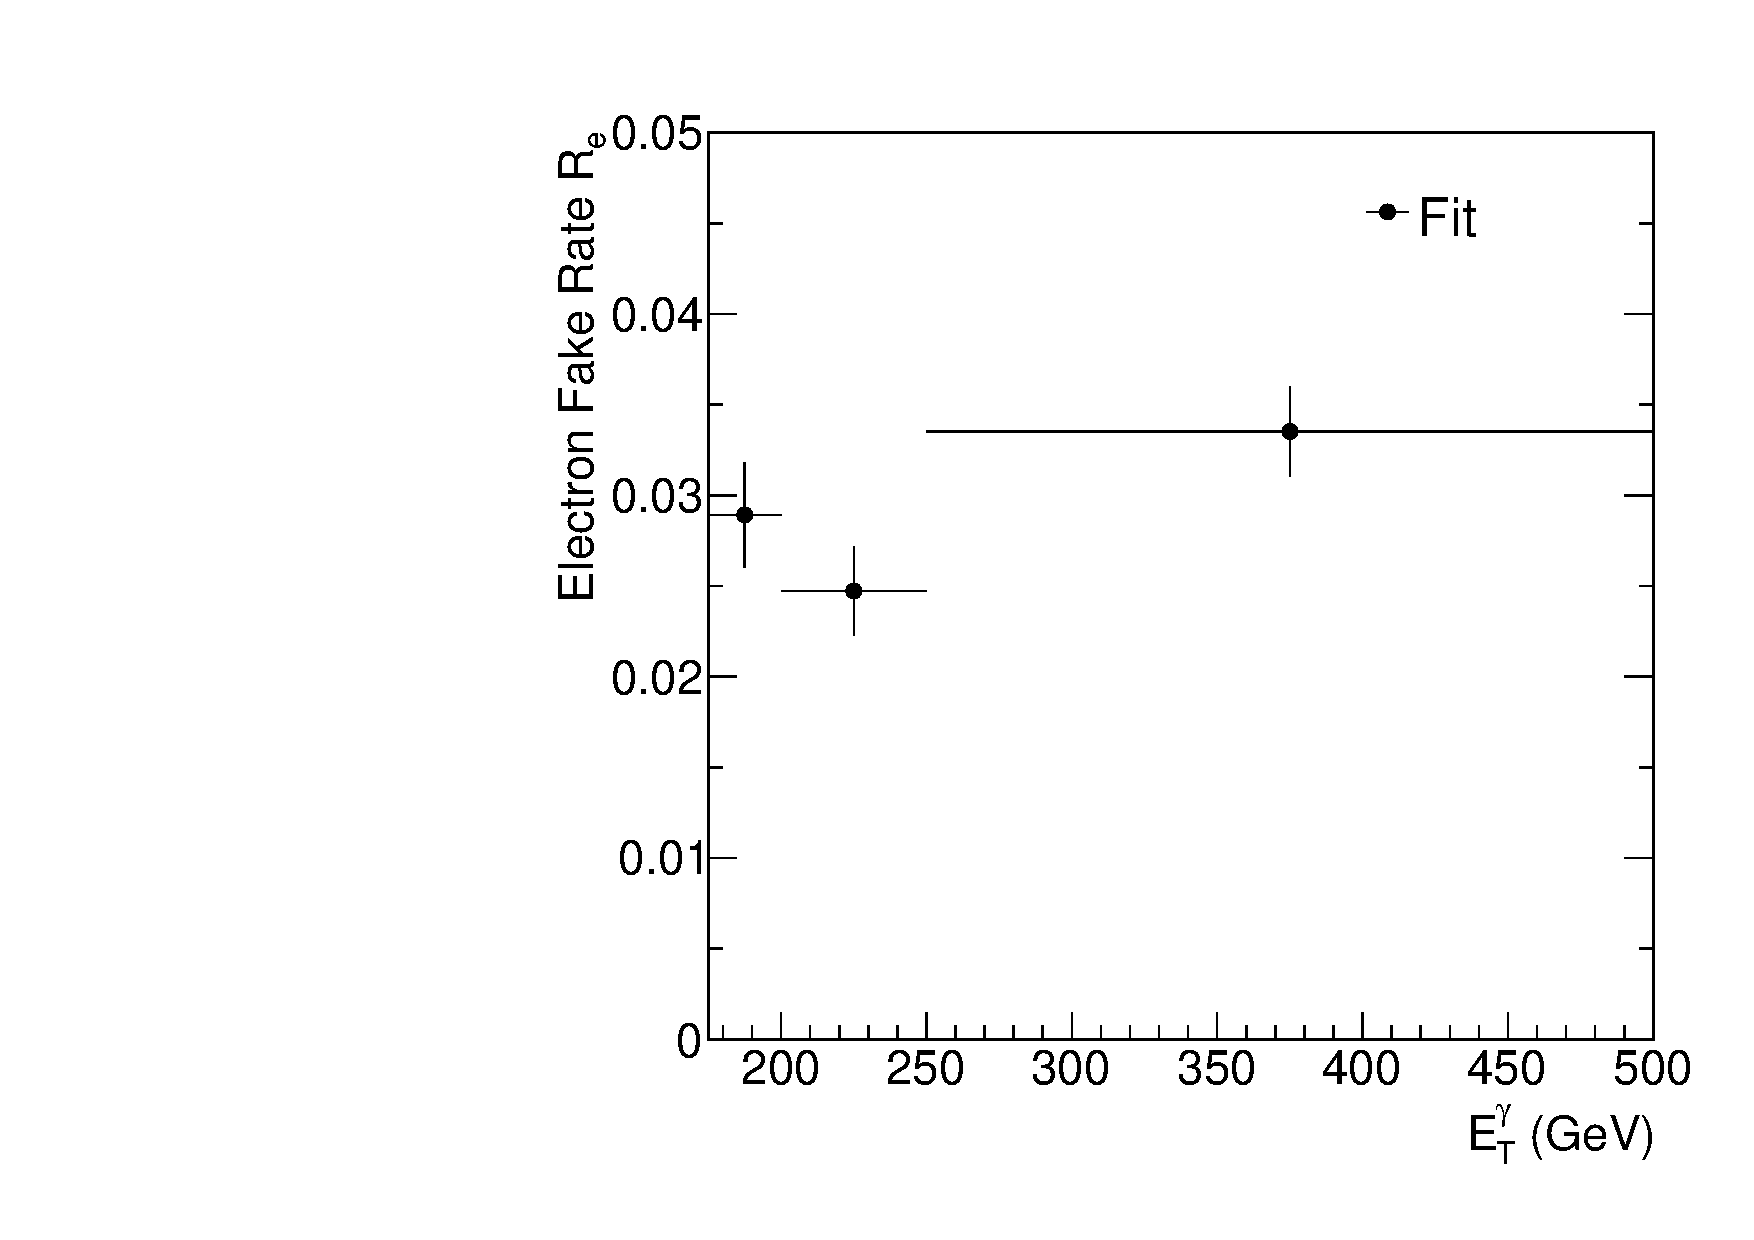
\includegraphics[width=0.5\textwidth]{Analysis/Figures/efake/frate_data_ptalt.pdf} 
    \caption{
      Electron to photon fake rate $R_{\Pe}$.
    }
    \label{fig:efake_frate}
\end{figure}


Figure~\ref{fig:efake_fits} shows the six fits performed on \Pe\Pe\ and \Pe\Pgg\ in bins of probe $\pt$, from which the $R_{\Pe}$ factor used for the estimation of the electron misidentification background is derived.
Figure~\ref{fig:efake_frate} shows the derived $R_{\Pe}$ factor as a function of \ETg. 
The electron proxy sample is reweighted by $R_{\Pe}$ depending on the \pt\ of the electron proxy object.

